\appendix
\chapter{Additional figures}
\label{A1}
% remove comment if you wish to add Appendix to contentsline.
%\addcontentsline{toc}{chapter}{Appendix A: How to download ERA5 data}

\section{HTI before and after fix of erroneous forecast}
\begin{figure}[H]
    \begin{subfigure}{0.45\textwidth}
    \centering
    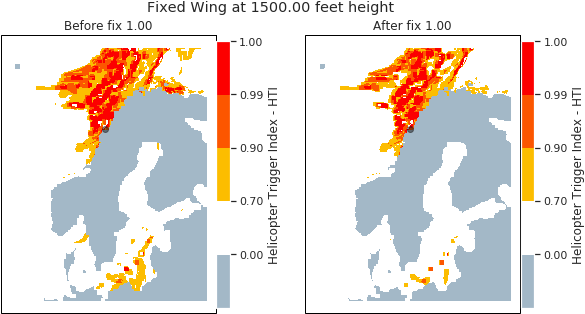
\includegraphics[width=\textwidth]{Figures/03.png}
    \caption{}
    \label{fig:HTI03}
    \end{subfigure}
    \hfill
    \begin{subfigure}{0.45\textwidth}
    \centering
    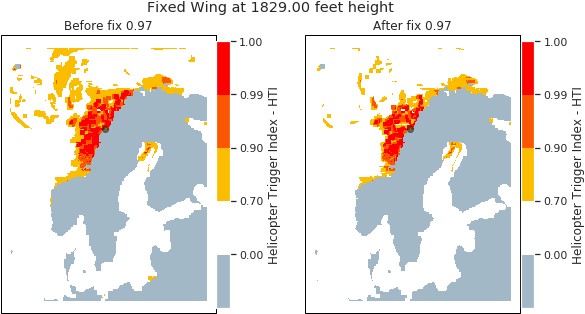
\includegraphics[width=\textwidth]{Figures/08.png}
    \caption{}
    \label{fig:HTI08}
    \end{subfigure}

    \begin{subfigure}{0.45\textwidth}
    \centering
    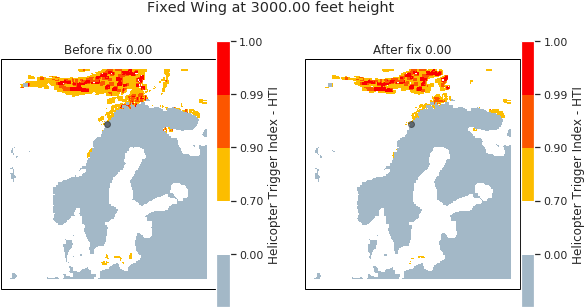
\includegraphics[width=\textwidth]{Figures/18.png}
    \caption{}
    \label{fig:HTI18}
    \end{subfigure}
\hfill
    \begin{subfigure}{0.45\textwidth}
    \centering
    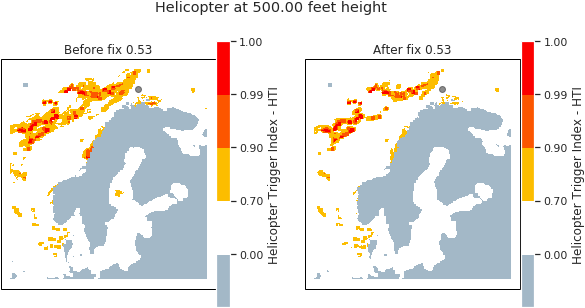
\includegraphics[width=\textwidth]{Figures/19.png}
    \caption{}
    \label{fig:HTI19}
    \end{subfigure}

    \begin{subfigure}{0.45\textwidth}
    \centering
    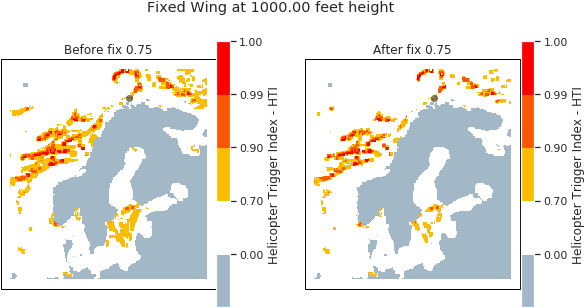
\includegraphics[width=\textwidth]{Figures/20.png}
    \caption{}
    \label{fig:HTI20}
    \end{subfigure}
\hfill
    \begin{subfigure}{0.45\textwidth}
    \centering
    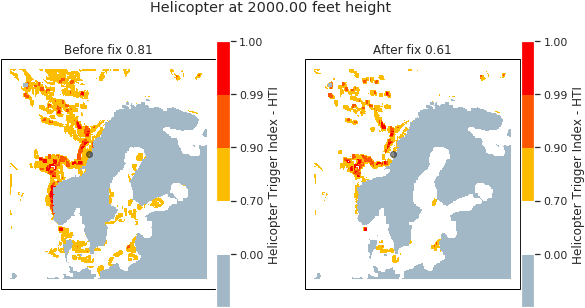
\includegraphics[width=\textwidth]{Figures/25.png}
    \caption{}
    \label{fig:HTI25}
    \end{subfigure}
    \centering
    \begin{subfigure}{0.45\textwidth}
    \centering
    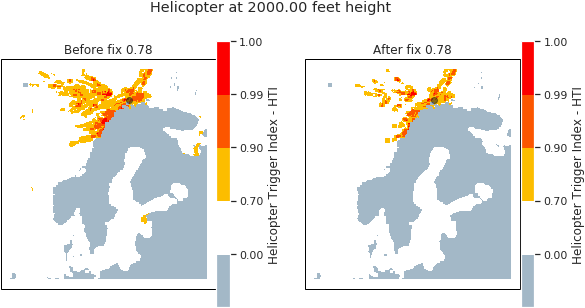
\includegraphics[width=\textwidth]{Figures/29.png}
    \caption{}
    \label{fig:HTI29}
    \end{subfigure}
\caption{North zone, cases with HTI-value before and after precipitation change}
\end{figure}

\begin{figure}[H]
    \begin{subfigure}{0.45\textwidth}
    \centering
    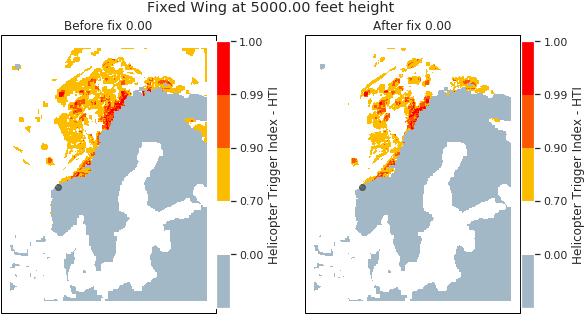
\includegraphics[width=\textwidth]{Figures/05.png}
    \caption{}
    \label{fig:HTI05}
    \end{subfigure}
    \hfill
    \begin{subfigure}{0.45\textwidth}
    \centering
    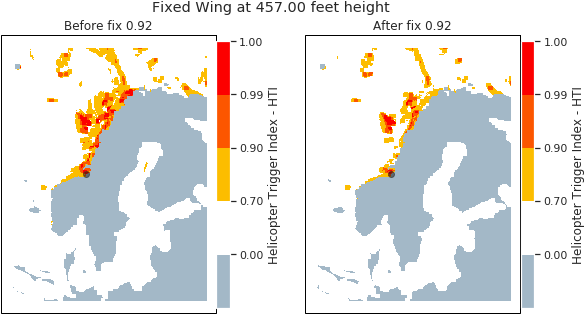
\includegraphics[width=\textwidth]{Figures/06.png}
    \caption{}
    \label{fig:HTI06}
    \end{subfigure}
    
    \begin{subfigure}{0.45\textwidth}
    \centering
    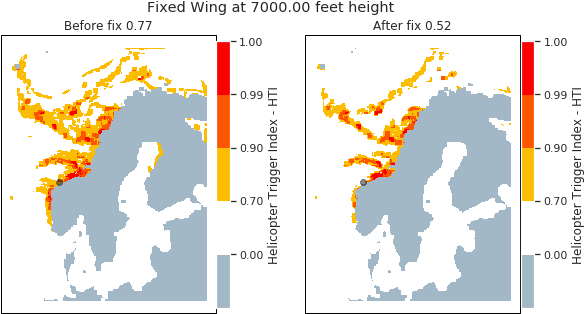
\includegraphics[width=\textwidth]{Figures/09.png}
    \caption{}
    \label{fig:HTI09}
    \end{subfigure}
\hfill
    \begin{subfigure}{0.45\textwidth}
    \centering
    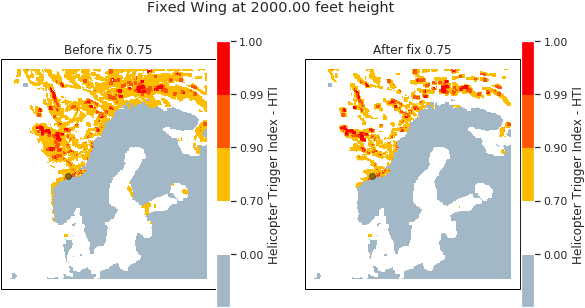
\includegraphics[width=\textwidth]{Figures/11.png}
    \caption{}
    \label{fig:HTI11}
    \end{subfigure}
    
    \begin{subfigure}{0.45\textwidth}
    \centering
    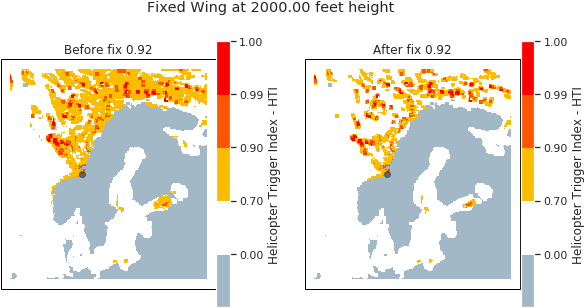
\includegraphics[width=\textwidth]{Figures/12.png}
    \caption{}
    \label{fig:HTI12}
    \end{subfigure}
\hfill
    \begin{subfigure}{0.45\textwidth}
    \centering
    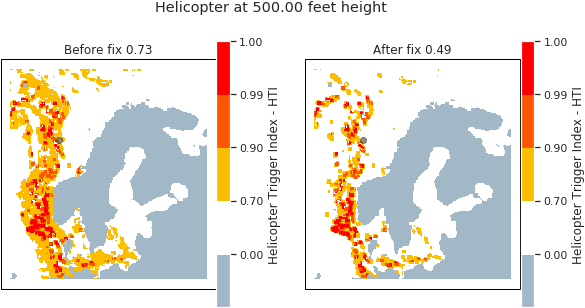
\includegraphics[width=\textwidth]{Figures/21.png}
    \caption{}
    \label{fig:HTI21}
    \end{subfigure}

    \begin{subfigure}{0.45\textwidth}
    \centering
    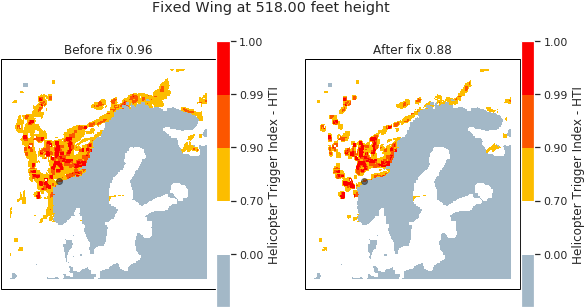
\includegraphics[width=\textwidth]{Figures/22.png}
    \caption{}
    \label{fig:HTI22}
    \end{subfigure}
\hfill
    \begin{subfigure}{0.45\textwidth}
    \centering
    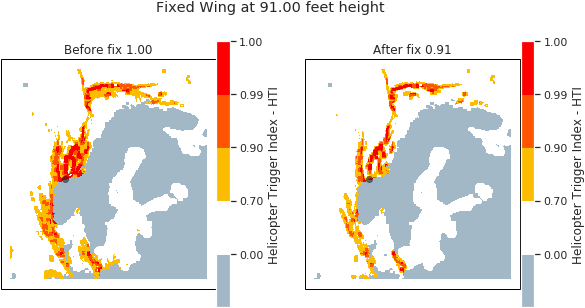
\includegraphics[width=\textwidth]{Figures/34.png}
    \caption{}
    \label{fig:HTI34}
    \end{subfigure}
\caption{North West zone, cases with HTI-value before and after precipitation change}
\end{figure}


\begin{figure}[H]
    \begin{subfigure}{0.45\textwidth}
    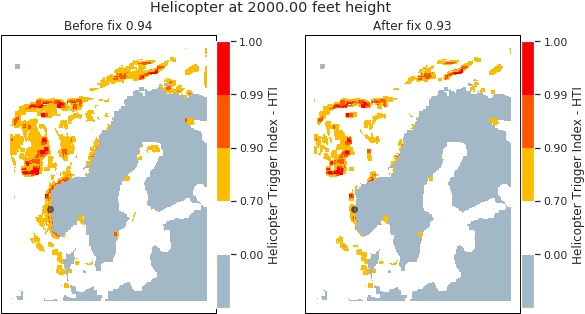
\includegraphics[width=\textwidth]{Figures/00.png}
    \caption{}
    \label{fig:HTI00}
    \end{subfigure}
\hfill
    \begin{subfigure}{0.45\textwidth}
    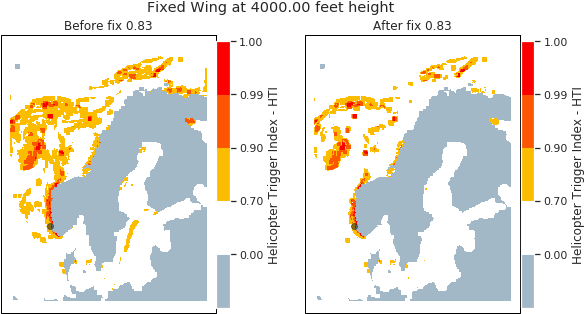
\includegraphics[width=\textwidth]{Figures/01.png}
    \caption{}
    \label{fig:HTI01}
    \end{subfigure}

    \begin{subfigure}{0.45\textwidth}
    \centering
    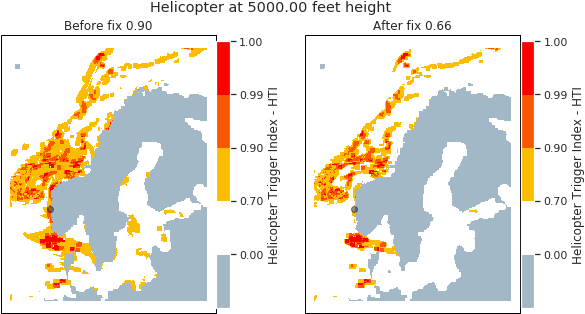
\includegraphics[width = \textwidth]{Figures/02.png}
    \caption{}
    \label{fig:HTI02}
    \end{subfigure}
\hfill
    \begin{subfigure}{0.45\textwidth}
    \centering
    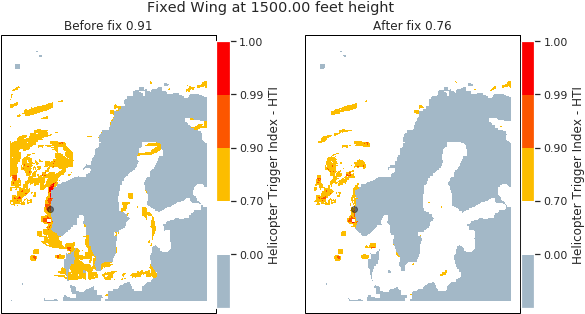
\includegraphics[width=\textwidth]{Figures/04.png}
    \caption{}
    \label{fig:HTI04}
    \end{subfigure}

    \begin{subfigure}{0.45\textwidth}
    \centering
    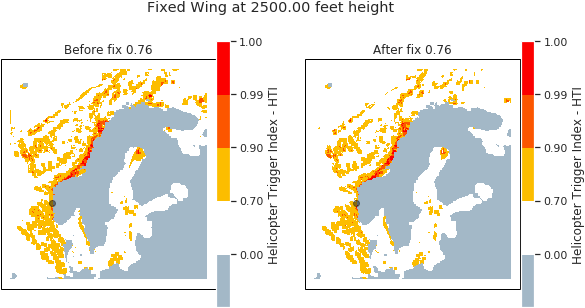
\includegraphics[width=\textwidth]{Figures/10.png}
    \caption{}
    \label{fig:HTI10}
    \end{subfigure}
\hfill
    \begin{subfigure}{0.45\textwidth}
    \centering
    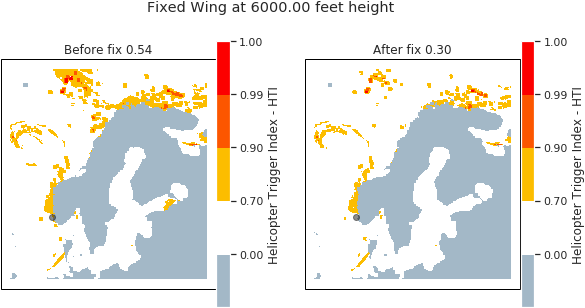
\includegraphics[width=\textwidth]{Figures/13.png}
    \caption{}
    \label{fig:HTI13}
    \end{subfigure}

    \begin{subfigure}{0.45\textwidth}
    \centering
    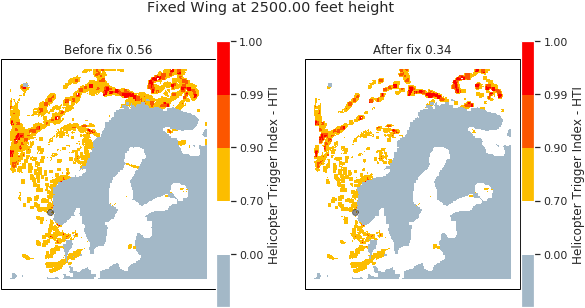
\includegraphics[width=\textwidth]{Figures/14.png}
    \caption{}
    \label{fig:HTI14}
    \end{subfigure}
\hfill
    \begin{subfigure}{0.45\textwidth}
    \centering
    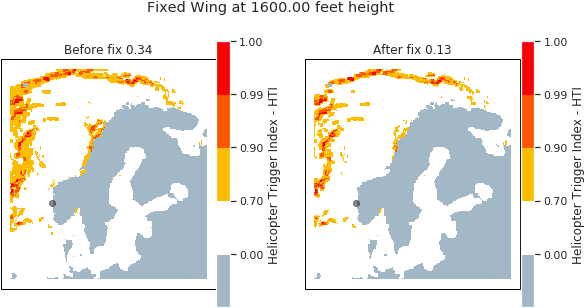
\includegraphics[width=\textwidth]{Figures/15.png}
    \caption{}
    \label{fig:HTI15}
    \end{subfigure}
\caption{West zone (First part), cases with HTI-value before and after precipitation change}
\end{figure}

\begin{figure}[H]
    \begin{subfigure}{0.45\textwidth}
    \centering
    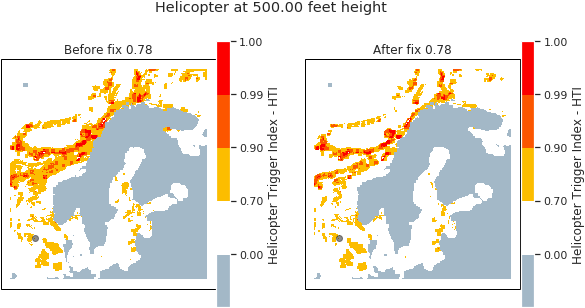
\includegraphics[width=\textwidth]{Figures/16.png}
    \caption{}
    \label{fig:HTI16}
    \end{subfigure}
\hfill
    \begin{subfigure}{0.45\textwidth}
    \centering
    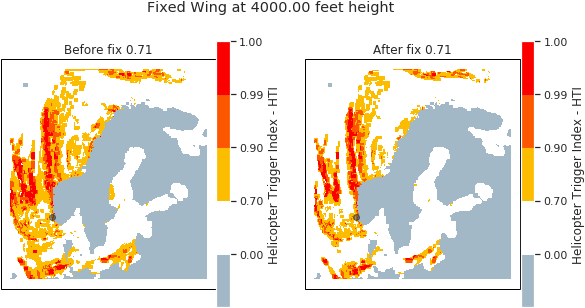
\includegraphics[width=\textwidth]{Figures/17.png}
    \caption{}
    \label{fig:HTI17}
    \end{subfigure}

    \begin{subfigure}{0.45\textwidth}
    \centering
    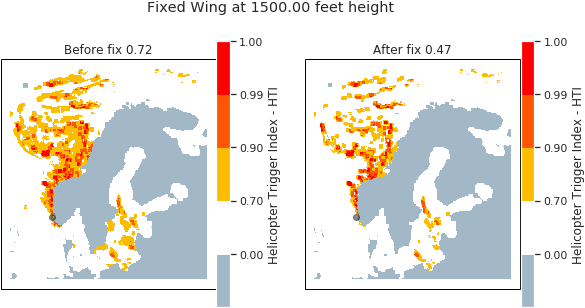
\includegraphics[width=\textwidth]{Figures/23.png}
    \caption{}
    \label{fig:HTI23}
    \end{subfigure}
\hfill
    \begin{subfigure}{0.45\textwidth}
    \centering
    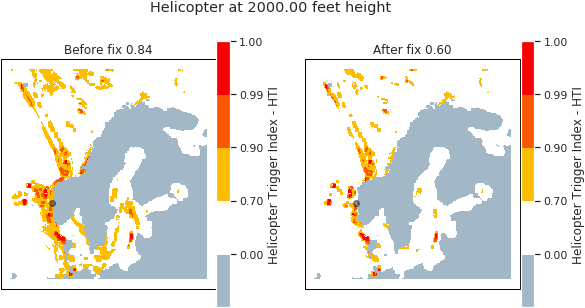
\includegraphics[width=\textwidth]{Figures/24.png}
    \caption{}
    \label{fig:HTI24}
    \end{subfigure}

    \begin{subfigure}{0.45\textwidth}
    \centering
    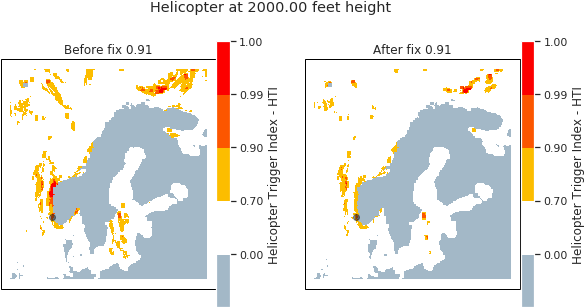
\includegraphics[width=\textwidth]{Figures/26.png}
    \caption{}
    \label{fig:HTI26}
    \end{subfigure}
\hfill
    \begin{subfigure}{0.45\textwidth}
    \centering
    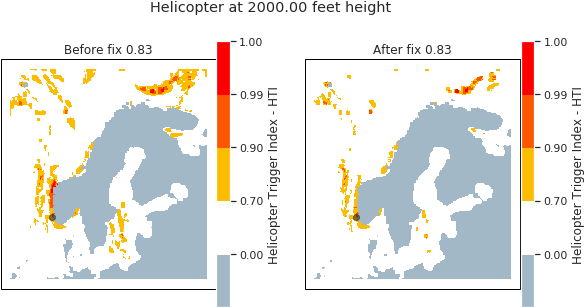
\includegraphics[width=\textwidth]{Figures/27.png}
    \caption{}
    \label{fig:HTI27}
    \end{subfigure}

    \begin{subfigure}{0.45\textwidth}
    \centering
    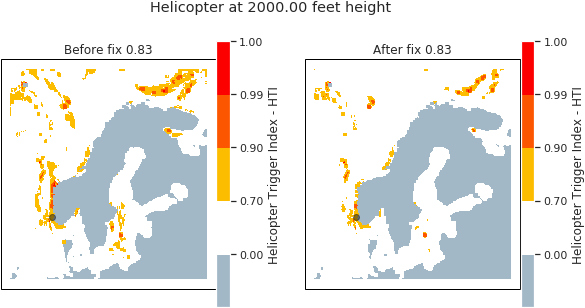
\includegraphics[width=\textwidth]{Figures/28.png}
    \caption{}
    \label{fig:HTI28}
    \end{subfigure}
\hfill
    \begin{subfigure}{0.45\textwidth}
    \centering
    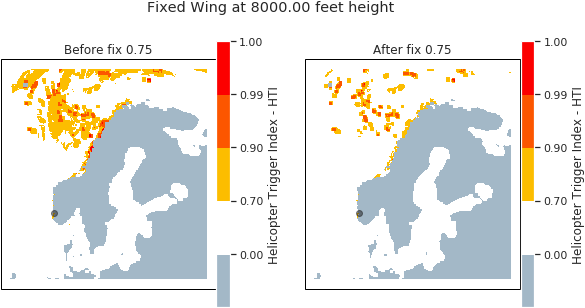
\includegraphics[width=\textwidth]{Figures/32.png}
    \caption{}
    \label{fig:HTI32}
    \end{subfigure}
\centering
    \begin{subfigure}{0.45\textwidth}
    \centering
    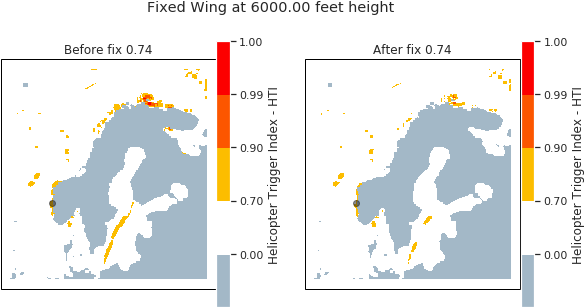
\includegraphics[width=\textwidth]{Figures/33.png}
    \caption{}
    \label{fig:HTI33}
    \end{subfigure}
\caption{West zone (Second part), cases with HTI-value before and after precipitation change}

\end{figure}

\begin{figure}[H]
    \begin{subfigure}{0.45\textwidth}
    \centering
    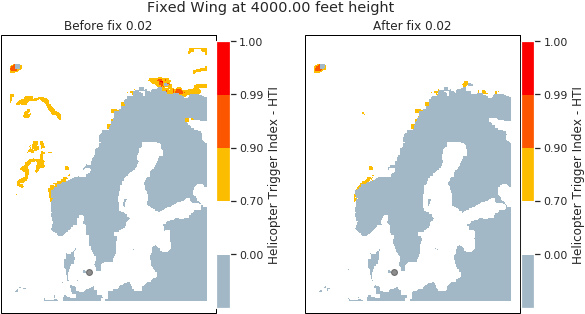
\includegraphics[width=\textwidth]{Figures/07.png}
    \caption{}
    \label{fig:HTI07}
    \end{subfigure}
\hfill
    \begin{subfigure}{0.45\textwidth}
    \centering
    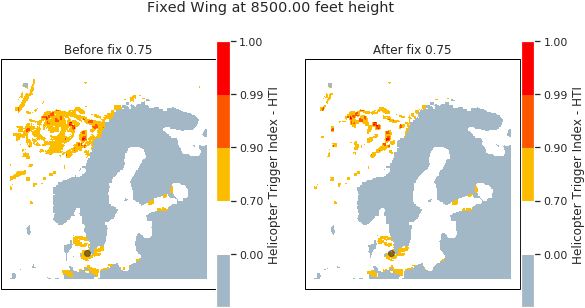
\includegraphics[width=\textwidth]{Figures/30.png}
    \caption{}
    \label{fig:HTI30}
    \end{subfigure}
    \centering
    \begin{subfigure}{0.45\textwidth}
    \centering
    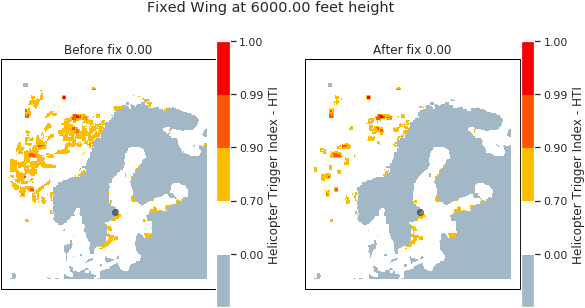
\includegraphics[width=\textwidth]{Figures/31.png}
    \caption{}
    \label{fig:HTI31}
    \end{subfigure}
\caption{South zone, cases with HTI-value before and after precipitation change}
\end{figure}


\begin{figure}[H]
    \begin{subfigure}{0.45\textwidth}
    \centering
    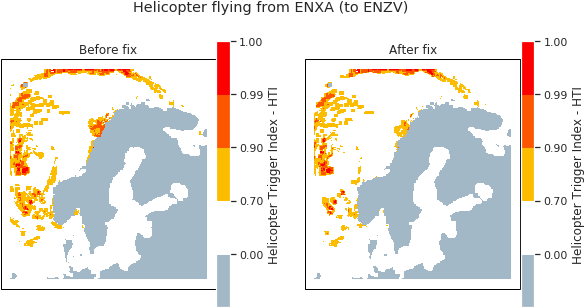
\includegraphics[width=\textwidth]{Figures/Analysis00.png}
    \caption{}
    \label{fig:HTIA00}
    \end{subfigure}
\hfill
    \begin{subfigure}{0.45\textwidth}
    \centering
    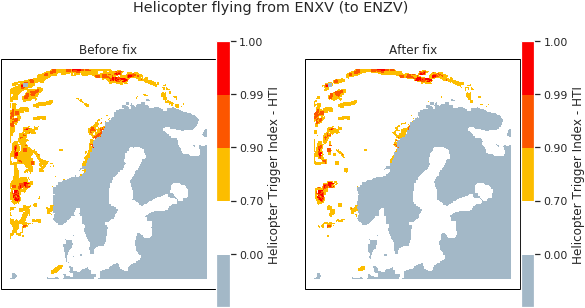
\includegraphics[width=\textwidth]{Figures/Analysis01.png}
    \caption{}
    \label{fig:HTIA01}
    \end{subfigure}

    \begin{subfigure}{0.45\textwidth}
    \centering
    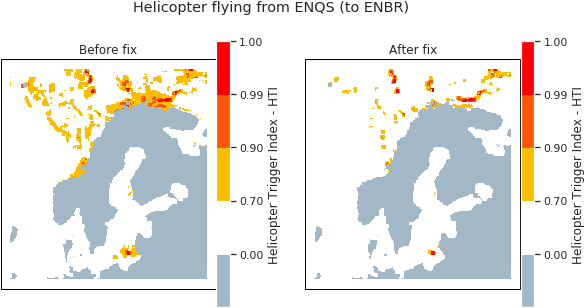
\includegraphics[width=\textwidth]{Figures/Analysis02.png}
    \caption{}
    \label{fig:HTIA02}
    \end{subfigure}
\hfill
    \begin{subfigure}{0.45\textwidth}
    \centering
    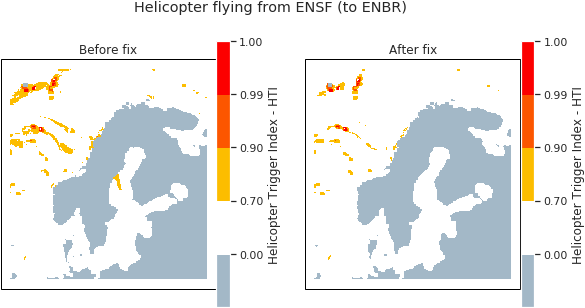
\includegraphics[width=\textwidth]{Figures/Analysis03.png}
    \caption{}
    \label{fig:HTIA03}
    \end{subfigure}

    \begin{subfigure}{0.45\textwidth}
    \centering
    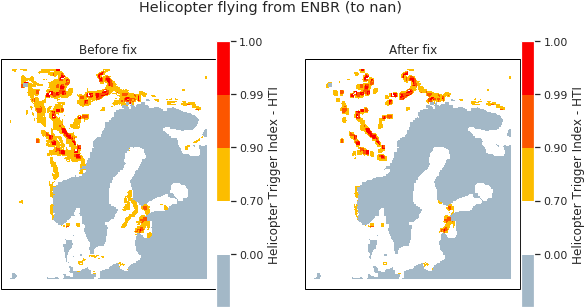
\includegraphics[width=\textwidth]{Figures/Analysis04.png}
    \caption{}
    \label{fig:HTIA04}
    \end{subfigure}
\hfill
    \begin{subfigure}{0.45\textwidth}
    \centering
    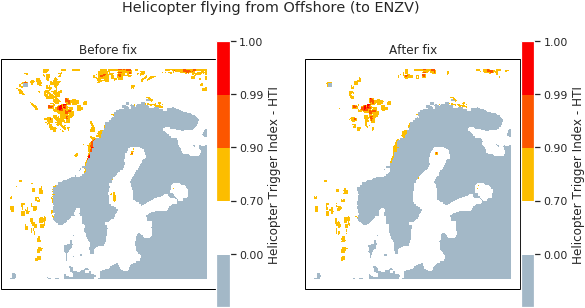
\includegraphics[width=\textwidth]{Figures/Analysis05.png}
    \caption{}
    \label{fig:HTIA05}
    \end{subfigure}
\caption{Cases where exact position is not-known, with HTI-value before and after precipitation change}

\end{figure}

\section{Cloud cover composites from ERA5}

\begin{figure}
\begin{subfigure}[b]{0.49\textwidth}
    \centering
    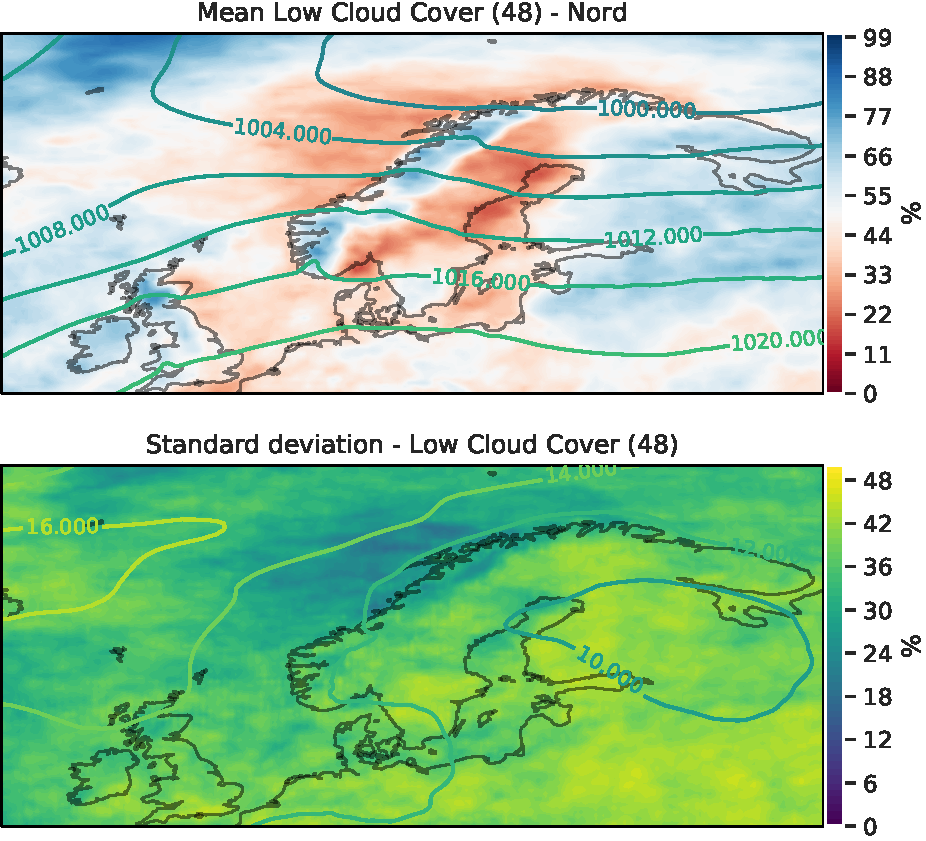
\includegraphics[width=\textwidth]{Figures/CCNord.pdf}
    \caption{Temperature for cases in North zone.}
    \label{fig:NordCC}
\end{subfigure}
\begin{subfigure}[b]{0.49\textwidth}
    \centering
    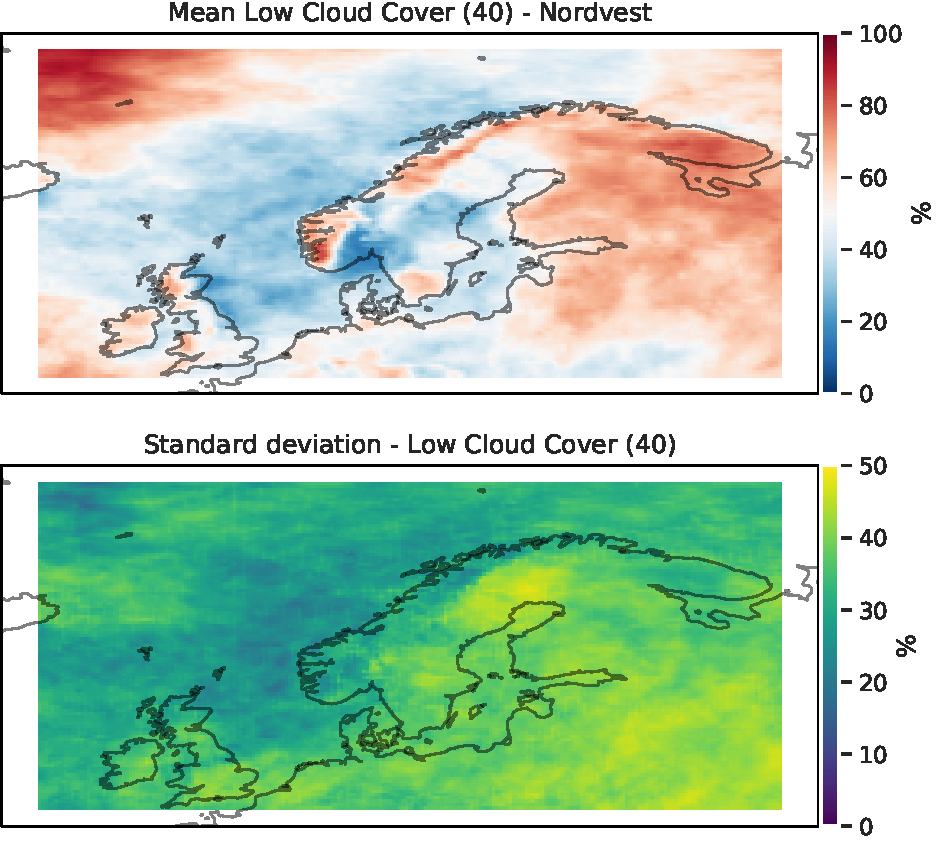
\includegraphics[width=\textwidth]{Figures/CCNordvest.pdf}
    \caption{Temperature for cases in Northwest zone.}
    \label{fig:NordWestCC}
\end{subfigure}
\begin{subfigure}[b]{0.49\textwidth}
    \centering
    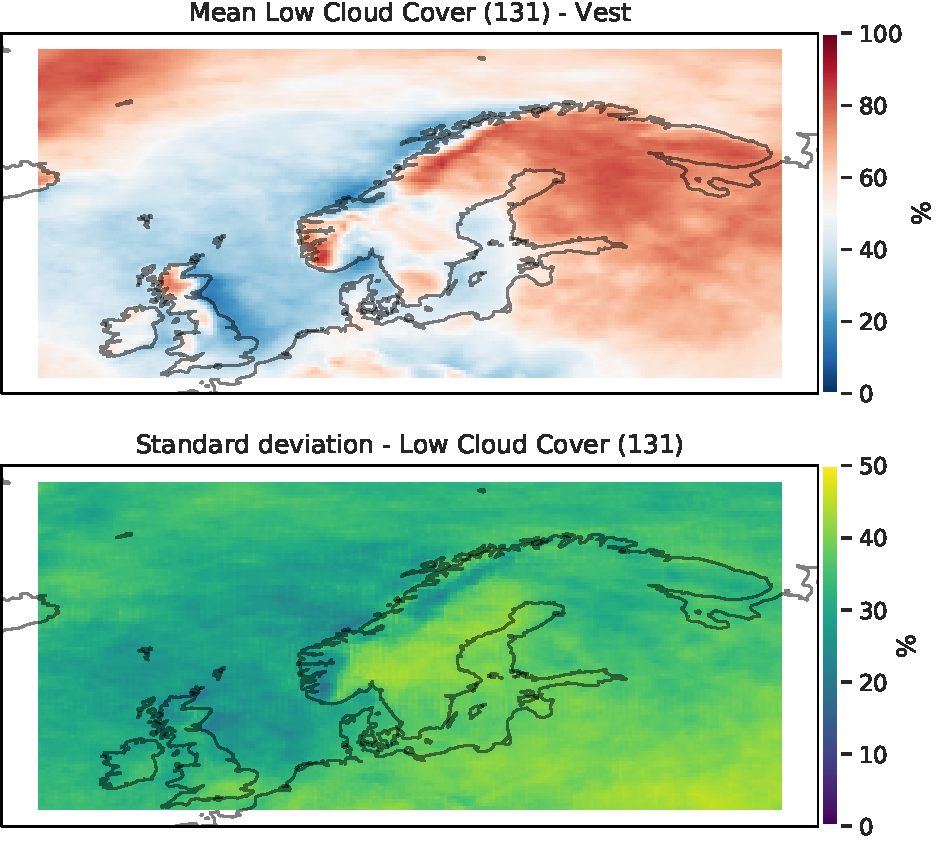
\includegraphics[width=\textwidth]{Figures/CCVest.pdf}
    \caption{Temperature for cases in West zone.}
    \label{fig:WestCC}
\end{subfigure}
\begin{subfigure}[b]{0.49\textwidth}
    \centering
    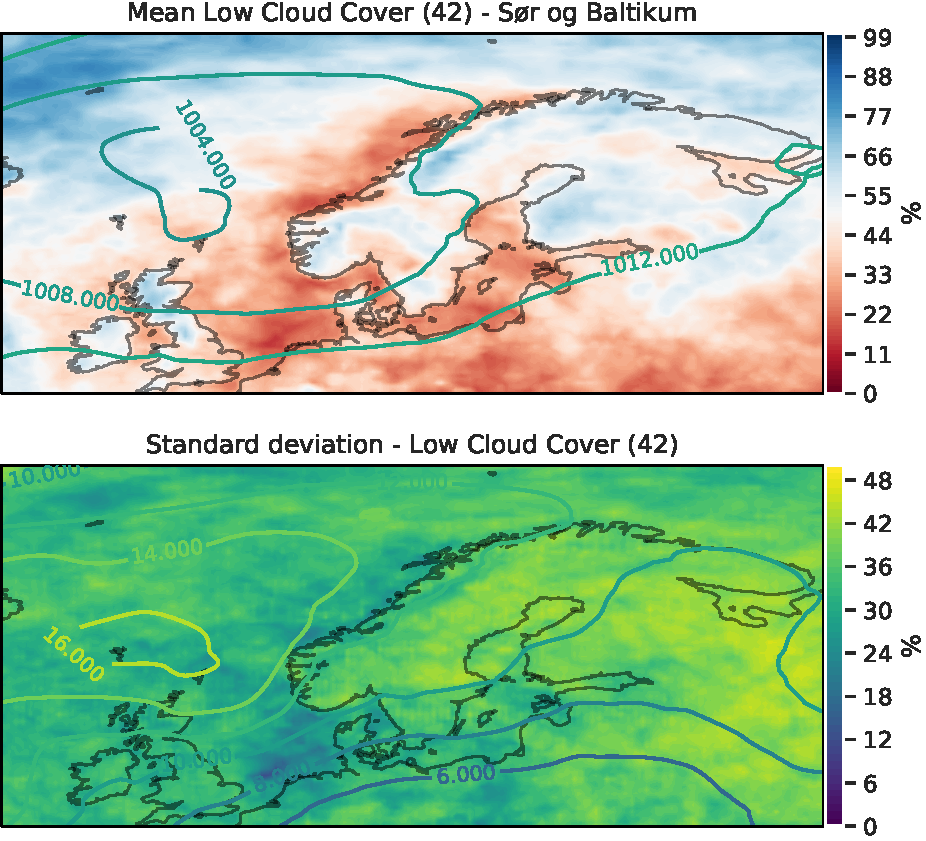
\includegraphics[width=\textwidth]{Figures/CCSor.pdf}
    \caption{Temperature for cases in South zone.}
    \label{fig:SouthCC}
\end{subfigure}
\caption{}
\label{fig:cloudcoverzones}
\end{figure}

\begin{figure}
     \centering
     \begin{subfigure}[b]{0.49\textwidth}
         \centering
         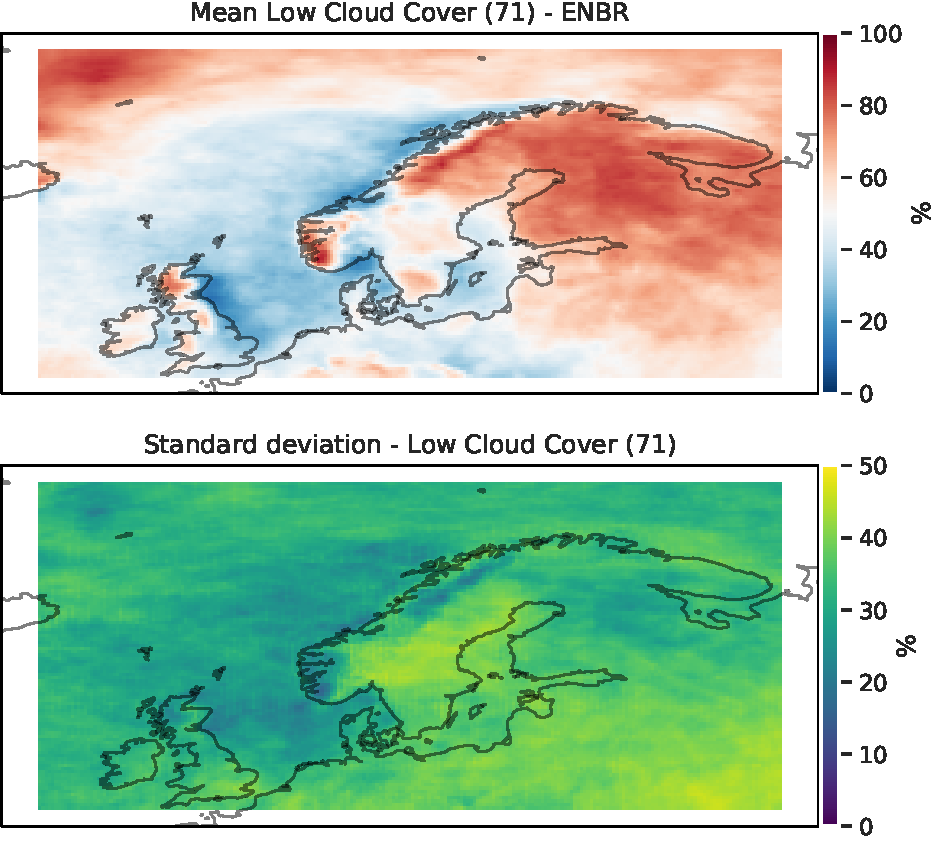
\includegraphics[width=\textwidth]{Figures/CCENBR.pdf}
         \caption{Cloud cover for cases at Flesland}
         \label{fig:ENBRCC}
     \end{subfigure}
     \hfill
     \begin{subfigure}[b]{0.49\textwidth}
         \centering
         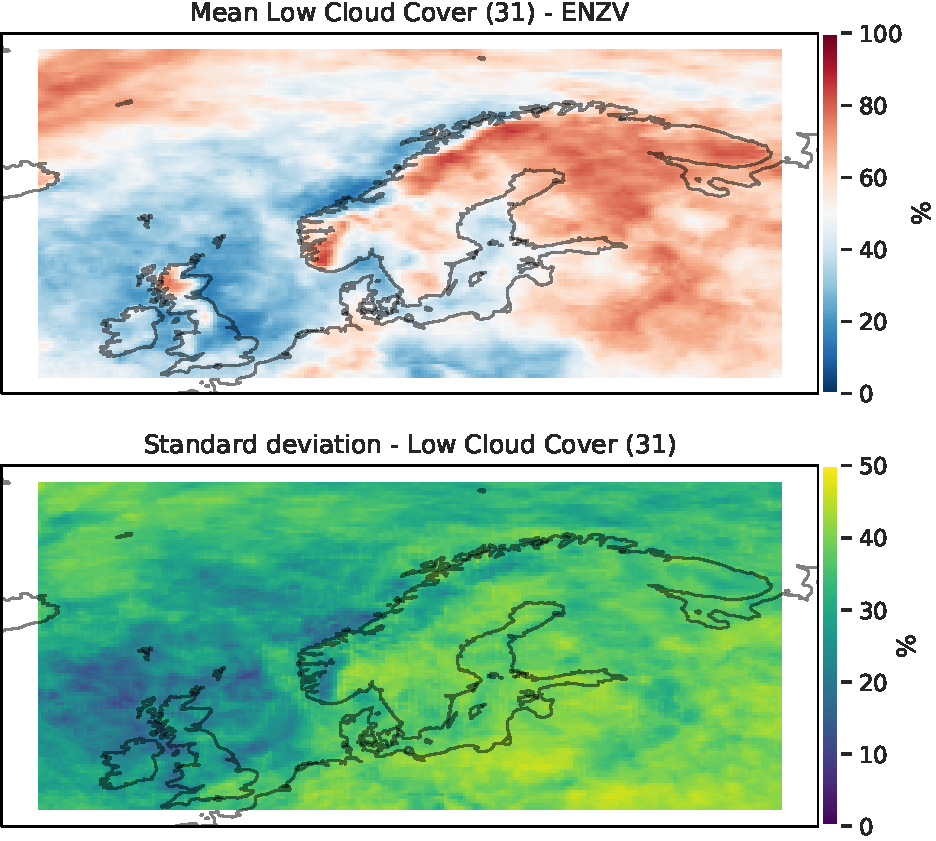
\includegraphics[width=\textwidth]{Figures/CCENZV.pdf}
         \caption{Cloud cover for cases at Sola}
         \label{fig:ENZVCC}
     \end{subfigure}
     
    \begin{subfigure}[b]{0.5\textwidth}
    \centering
    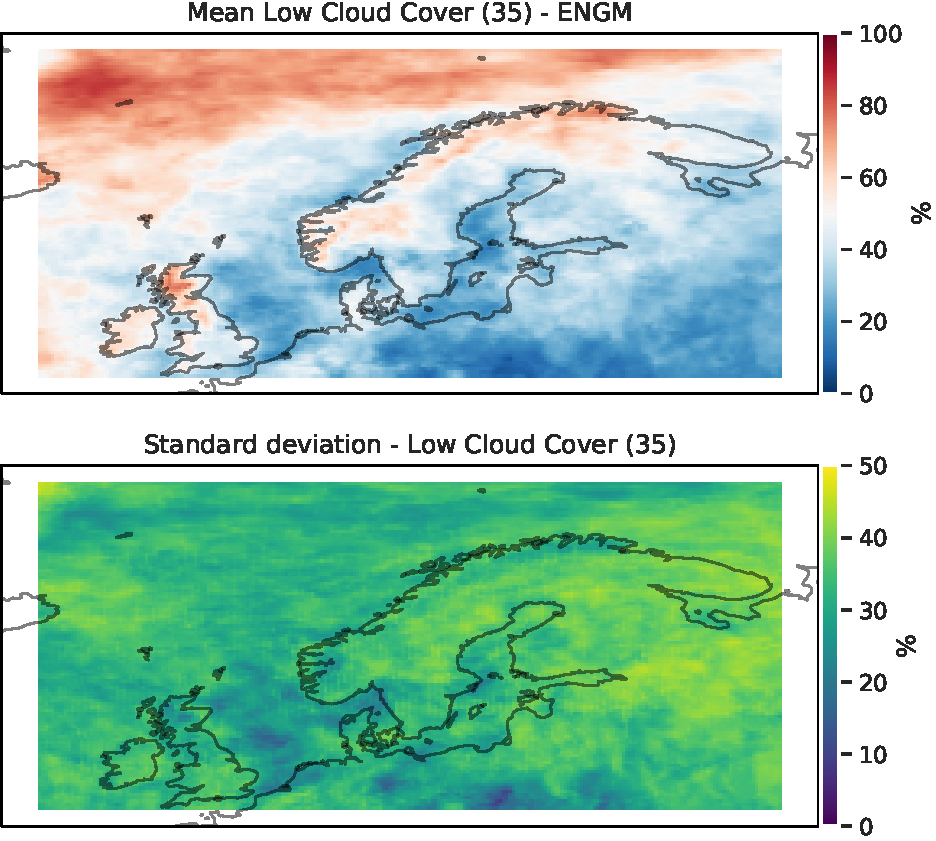
\includegraphics[width=\textwidth]{Figures/CCENGM.pdf}
    \caption{Cloud cover for cases at Gardermoen.}
    \label{fig:ENGMCC}
\end{subfigure}
\caption{ }
\label{fig:cloudcoverairports}
\end{figure}

\cleardoublepage


\chapter{Airport delineation and classification}

\begin{sidewaysfigure}
    \centering
    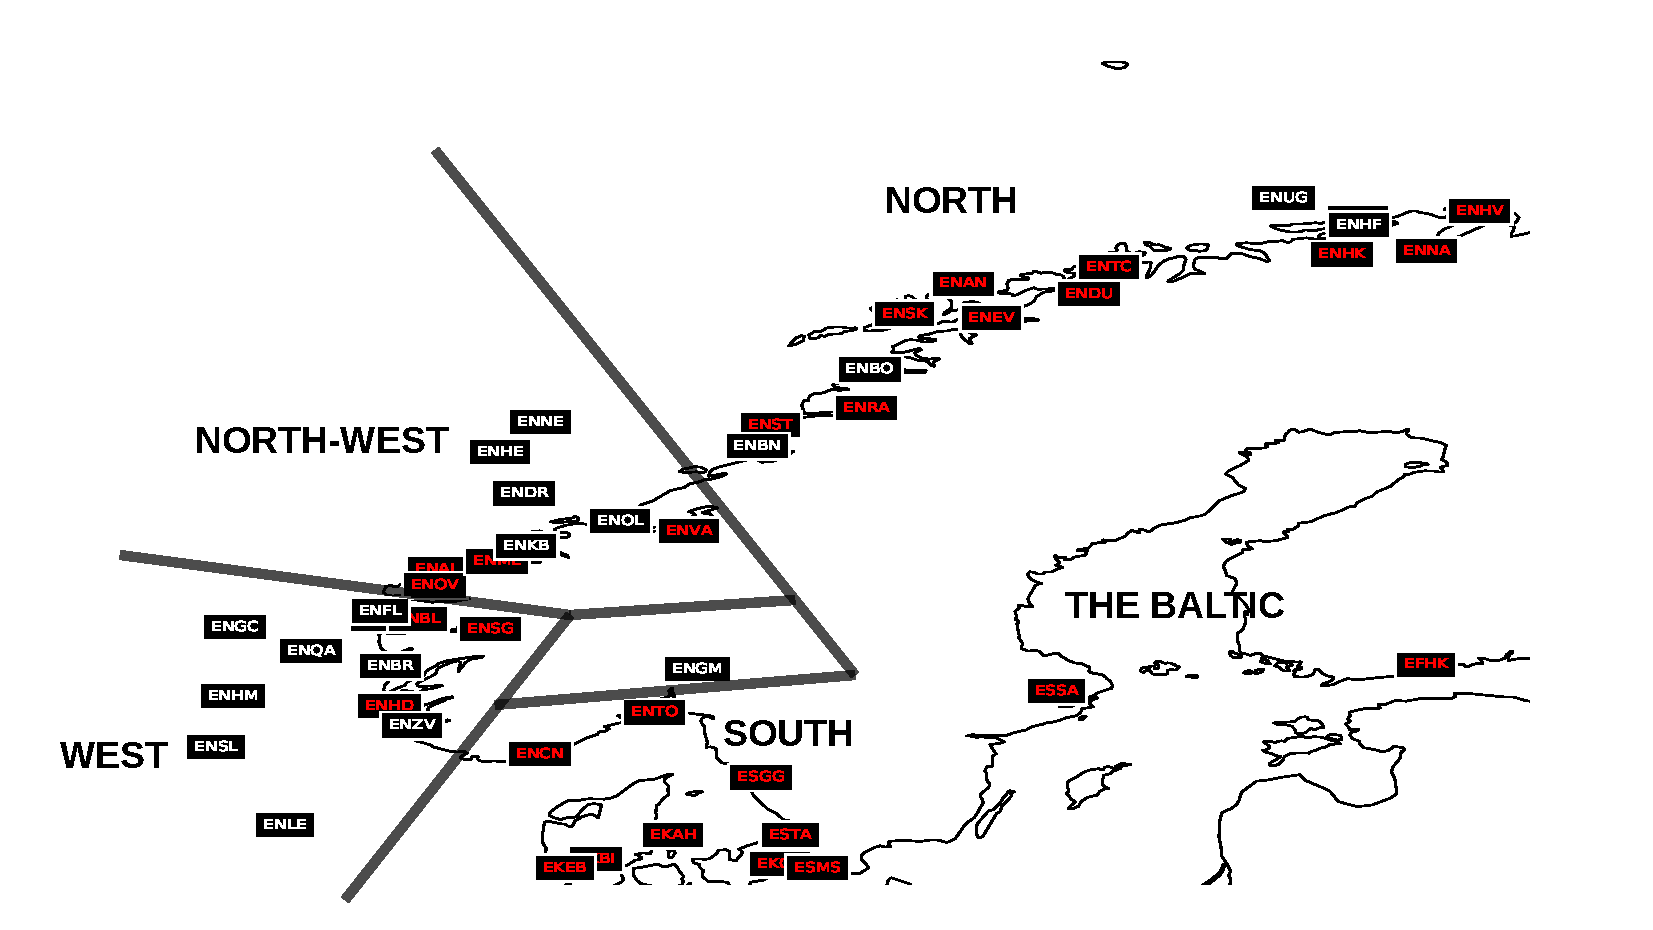
\includegraphics[width=\textwidth]{Figures/METARandHIT.pdf}
    \caption{Zones used in this thesis, with used METAR-stations in white, and airports with at least one incident in red.}
    \label{fig:Stationsmap}
\end{sidewaysfigure}

\section{ICAO-codes}

\begin{table}
    \begin{subtable}[h]{0.45\textwidth}
        \centering
         \begin{tabular}{r|l}
            ICAO-code & Airport name \\
            \hline
            ENGM & Gardermoen (Oslo) \\
            ENBR & Flesland (Bergen) \\
            ENZV & Sola (Stavanger)  \\
            ENKB & Kvernberget (Kristiansund) \\
            ENFL & Florø \\
            ENBO & Bodø \\
            ENBN & Brønnøy (Brønnøysund) \\
            ENOL & Ørland \\
            ENHF & Hammerfest \\
            ENML & Årø (Molde)\\
            ENHV & Valan (Honningsvåg)\\
        \end{tabular}
    \end{subtable}
    \hfill
    \begin{subtable}[h]{0.45\textwidth}
        \centering
        \begin{tabular}{r|l}
            ICAO-code & Offshore installation\\
            \hline
            ENXA &  Ekofisk A\\
            ENLE &  Ekofisk L\\
            ENXV &  Varg\\
            ENSF &  Statfjord A\\
            ENQS &  Statfjord C\\
            ENUG &  Goliat FPSO\\
            ENNE &  Norne A\\
            ENHE &  Heidrun A\\
            ENDR &  Draugen\\
            ENQA &  Troll A\\
            ENGC &  Gullfaks C\\
            ENHM &  Heimdal\\
            ENSL &  Sleipner A\\
        \end{tabular}
     \end{subtable}
    \caption{ICAO-code for the airports and helipads used in this thesis.}
    \label{tab:ICAO-table}
\end{table}